\documentclass[aspectratio=169]{beamer}
\usepackage{beamerthemeTealOceanPdflatex} % Custom theme with oceanic colors

% Enable notes on second screen (CHANGE THIS LINE)
\setbeameroption{show notes on second screen}

\usepackage{tikz}
\usetikzlibrary{angles, quotes, shapes.geometric, arrows.meta, positioning}
\tikzstyle{block} = [rectangle, rounded corners, minimum width=3cm, minimum height=1cm,text centered, draw=black, fill=blue!10]
\tikzstyle{arrow} = [thick, ->, >=Stealth]

% Additional packages for better presentation
\usepackage{booktabs}
\usepackage{amsmath}
\usepackage{amssymb}

% Custom commands for consistency
\newcommand{\highlight}[1]{\textbf{\color{accent2}#1}}
\newcommand{\tech}[1]{\texttt{#1}}

\title{Book Recommender using NLP}
\author{Carsten Lydeking}
\institute{Zealand Business College}
\date{Oral Exam -- AI and ML, 4th Semester}

\graphicspath{{../synopsis/figures/}}

\begin{document}

% Title slide
\begin{frame}
  \titlepage
  \note{
    \textbf{OPENING (30 seconds):}
    \begin{itemize}
      \item Good morning, I'm Carsten
      \item Book recommender using NLP for oral exam
      \item 10 min presentation + questions
      \item Focus on concepts and implementation
    \end{itemize}
  }
\end{frame}

% Main presentation slides
\begin{frame}{Motivation and Problem}
\begin{itemize}
  \item Increasing demand for privacy-preserving, local-first ML applications.
  \item Typical recommender systems rely on cloud APIs and user profiles.
  \item Goal: explore feasibility of a fully offline, content-based book recommender system.
  \item Research question:
    \begin{quote}
    How can a local ML model be used to recommend books based on natural language descriptions?
    \end{quote}
\end{itemize}
\end{frame}
\begin{frame}{Architecture Overview}
\begin{columns}[T]
  \begin{column}{0.50\textwidth}
	\textbf{Core Components:}
	\begin{itemize}
	  \item \highlight{Data Pipeline:} Clean \& augment book metadata
	  \item \highlight{Category Inference:} Zero-shot classification + fallback rules
	  \item \highlight{Semantic Embedding:} \tech{MiniLM} sentence transformers
	  \item \highlight{Vector Search:} \tech{FAISS} similarity matching
	  \item \highlight{Local UI:} \tech{Streamlit} interface
	\end{itemize}
	
	\vspace{0.1cm}
	\footnotesize \textbf{Key Innovation:} Fully local semantic search without cloud dependencies
  \end{column}
  
  \begin{column}{0.45\textwidth}
	\begin{center}
	  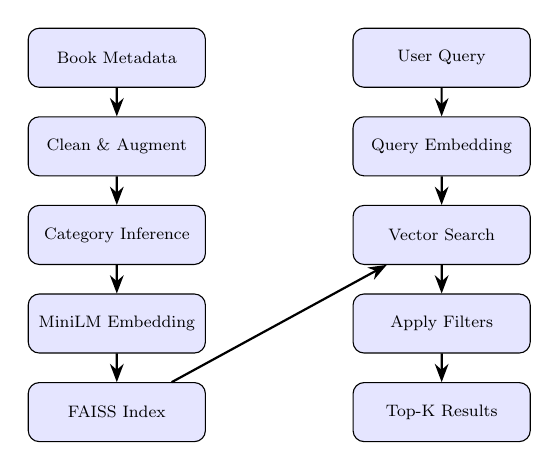
\begin{tikzpicture}[node distance=1.5cm, every node/.style={font=\footnotesize}, scale=0.75, transform shape]
		% Left pipeline (data processing)
		\node (desc) [block] {Book Metadata};
		\node (augment) [block, below of=desc] {Clean \& Augment};
		\node (classify) [block, below of=augment] {Category Inference};
		\node (embed) [block, below of=classify] {MiniLM Embedding};
		\node (index) [block, below of=embed] {FAISS Index};

		% Right pipeline (query processing)
		\node (query) [block, right of=desc, xshift=4cm] {User Query};
		\node (qembed) [block, below of=query] {Query Embedding};
		\node (search) [block, below of=qembed] {Vector Search};
		\node (filter) [block, below of=search] {Apply Filters};
		\node (output) [block, below of=filter] {Top-K Results};

		% Arrows
		\draw [arrow] (desc) -- (augment);
		\draw [arrow] (augment) -- (classify);
		\draw [arrow] (classify) -- (embed);
		\draw [arrow] (embed) -- (index);

		\draw [arrow] (query) -- (qembed);
		\draw [arrow] (qembed) -- (search);
		\draw [arrow] (index) -- (search);
		\draw [arrow] (search) -- (filter);
		\draw [arrow] (filter) -- (output);
	  \end{tikzpicture}
	\end{center}
  \end{column}
\end{columns}

\note{
  \begin{columns}[T]
	\begin{column}{0.49\textwidth}
	  [TIMING: 1 minute - DIAGRAM WALKTHROUGH:]
	  \begin{itemize}
		\item "Left side processes book data offline" (point to diagram)
		\item "Right side handles user queries in real-time"
		\item "Data flows from top to bottom, then connects for search"
		\item "Everything happens locally - no network calls"
	  \end{itemize}
	  
	  \vspace{0.2cm}
	  [DEFINE KEY TERMS:]
	  \begin{itemize}
		\item Zero-shot classification: "Model classifies without training examples - understands categories from descriptions alone"
		\item MiniLM: "Lightweight transformer model - like GPT but smaller, designed for understanding meaning"
		\item FAISS: "Facebook's library for fast similarity search - finds nearest neighbors in high-dimensional space"
		\item Semantic embedding: "Converting text to numbers that represent meaning - similar concepts get similar numbers"
	  \end{itemize}
	\end{column}
	  
	\begin{column}{0.49\textwidth}
		[KEY INNOVATION EMPHASIS:]
		\begin{itemize}
			\item "The innovation is making semantic search work locally and independently"
			\item "Usually requires cloud APIs like OpenAI or Google"
			\item "I prove you can do it on consumer hardware without dependencies"
		\end{itemize}
		
	\vspace{0.2cm}
	  [POTENTIAL QUESTIONS:]
	  \begin{itemize}
		\item \textit{"What's a transformer?"} → "Neural network architecture very good at understanding language context"
		\item \textit{"Why modular design?"} → "Easy to swap components, test approaches, maintain independence"
		\item \textit{"How does semantic differ from keyword search?"} → "Keywords match exact words, semantic understands concepts"
	  \end{itemize}
	  
	  \vspace{0.2cm}
	  [TRANSITION:]
	  \begin{itemize}
		\item "Let me dive into the data challenges I had to solve first..."
	  \end{itemize}
	\end{column}
  \end{columns}
}

\end{frame}
\begin{frame}{Dataset Exploration}
  
\begin{columns}[T]
  \centering
  \begin{column}{0.49\textwidth}
    Original dataset $\sim$ 6800 books
    \begin{itemize}
          \item Missing or inconsistent fields (authors, categories, descriptions)
          \item Very short or low-quality descriptions
          \item Category noise across sources
          \item OpenLibrary and Google Books API used to enrich metadata
          \item Rows with $<9$ words in description removed
          \item Final dataset: 5160 high-confidence books
        \end{itemize}
  \end{column}

  \begin{column}{0.49\textwidth}
  \centering
      \includegraphics[width=\textwidth]{reexp_mismatch_counts.png}
  \end{column}
\end{columns}
\end{frame}
\begin{frame}{Category Inference}

\begin{columns}
  % First column with text and bullet points
  \begin{column}{0.49\textwidth}
    \centering
    \begin{itemize}
      \item Zero-shot classification with BART-MNLI
      \item 13 candidate categories defined
      \item Fallback keyword rules added for weak predictions
      \item Per-category metrics calculated:
        \begin{itemize}
          \item Precision
          \item Recall
          \item F1-score
        \end{itemize}

      \item Final filtering based on confidence thresholds:
        \begin{itemize}
          \item description\_length $\geq$ 200 chars
          \item avg\_score $\geq$ 0.2
          \item max\_score $\geq$ 0.4
        \end{itemize}
  \end{itemize} 
  \end{column}

  \begin{column}{0.45\textwidth}
    \centering
    \includegraphics[width=\textwidth]{refine_category_metrics_plot.png}
  \end{column}
\end{columns}

\end{frame}

\begin{frame}{Semantic Embedding \& Vector Search}

\begin{columns}[T]
  \begin{column}{0.50\textwidth}
    \textbf{Sentence Embedding with \tech{MiniLM}:}
    \begin{itemize}
      \item \highlight{Model:} \tech{all-MiniLM-L6-v2}
      \item \highlight{Input format:} \\
        {\scriptsize \textit{"Title: ... Author: ... Description: ..."}}
      \item \highlight{Output:} 384-dimensional vectors
      \item \highlight{Advantage:} Semantic similarity beyond keywords
    \end{itemize}

    \vspace{0.3cm}
    \textbf{Vector Search with \tech{FAISS}:}
    \begin{itemize}
      \item \highlight{Index:} 5,160 book embeddings
      \item \highlight{Search:} L2 distance (exact search)
      \item \highlight{Performance:} $<$ 10ms query time
      \item \highlight{Local:} No external dependencies
    \end{itemize}
  \end{column}

  \begin{column}{0.45\textwidth}
    \centering
    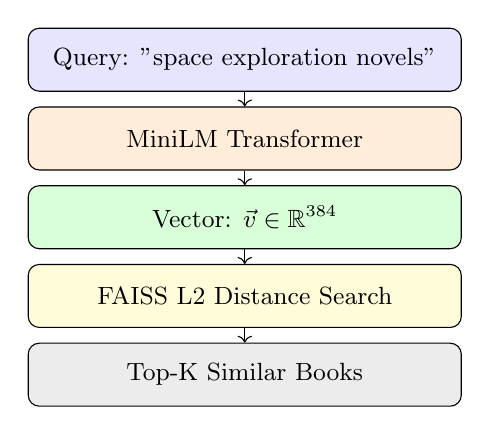
\begin{tikzpicture}[node distance=1.0cm, every node/.style={font=\small}]
        % Embedding process
        \node (input) [draw, rounded corners, minimum width=5.5cm, minimum height=0.8cm, fill=blue!10] 
        {\small Query: "space exploration novels"};

        \node (embed) [below of=input, draw, rounded corners, minimum width=5.5cm, minimum height=0.8cm, fill=orange!15] 
        {\small MiniLM Transformer};

        \node (vector) [below of=embed, draw, rounded corners, minimum width=5.5cm, minimum height=0.8cm, fill=green!15] 
        {\small Vector: $\vec{v} \in \mathbb{R}^{384}$};

        % Search process
        \node (faiss) [below of=vector, draw, rounded corners, minimum width=5.5cm, minimum height=0.8cm, fill=yellow!15] 
        {\small FAISS L2 Distance Search};

        \node (results) [below of=faiss, draw, rounded corners, minimum width=5.5cm, minimum height=0.8cm, fill=gray!15] 
        {\small Top-K Similar Books};

        % Arrows
        \draw[->] (input) -- (embed);
        \draw[->] (embed) -- (vector);
        \draw[->] (vector) -- (faiss);
        \draw[->] (faiss) -- (results);
    \end{tikzpicture}
    
    \vspace{0.2cm}
    \small \textit{End-to-end semantic search in $<$ 200ms}
  \end{column}
\end{columns}

\end{frame}
\begin{frame}{Vector Similarity Search with FAISS}

\begin{columns}[T]
  \begin{column}{0.45\textwidth}
    \begin{itemize}
        \item Used \textbf{Facebook AI Similarity Search (FAISS)} library
        \item Performs \textbf{L2 distance} search in embedding space
        \item Index built with:
          \begin{itemize}
            \item 5160 book embeddings (\( \vec{v} \in \mathbb{R}^{384} \))
            \item Exact search (IndexFlatL2)
          \end{itemize}
        \item At runtime:
          \begin{itemize}
            \item User query is embedded
            \item Top-k nearest neighbors retrieved
            \item Results shown in UI
          \end{itemize}
        \item \textbf{Fully local}, fast search
    \end{itemize}
  \end{column}

  \begin{column}{0.50\textwidth}
    \centering
    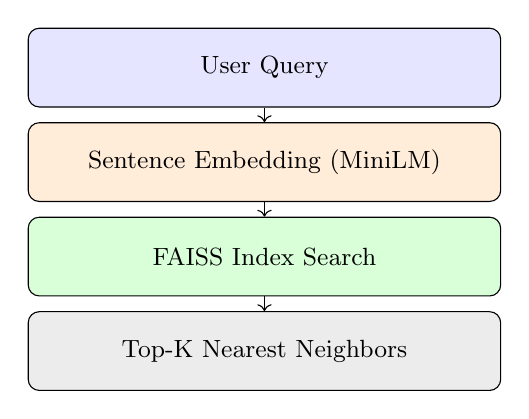
\begin{tikzpicture}[node distance=1.2cm, every node/.style={font=\small}]
        \node (query) [draw, rounded corners, minimum width=6cm, minimum height=1cm, fill=blue!10] {User Query};

        \node (embed) [below of=query, draw, rounded corners, minimum width=6cm, minimum height=1cm, fill=orange!15] {Sentence Embedding (MiniLM)};

        \node (faiss) [below of=embed, draw, rounded corners, minimum width=6cm, minimum height=1cm, fill=green!15] {FAISS Index Search};

        \node (results) [below of=faiss, draw, rounded corners, minimum width=6cm, minimum height=1cm, fill=gray!15] {Top-K Nearest Neighbors};

        \draw[->] (query) -- (embed);
        \draw[->] (embed) -- (faiss);
        \draw[->] (faiss) -- (results);
    \end{tikzpicture}
  \end{column}
\end{columns}

\end{frame}

\begin{frame}{Critical Analysis \& Future Directions}

\begin{columns}[T]
  \begin{column}{0.50\textwidth}
    \textbf{Implementation Strengths:}
    \begin{itemize}
      \item \highlight{Privacy-preserving} by design
      \item \highlight{Semantic understanding} beyond keyword matching
      \item \highlight{Lightweight} - runs on consumer hardware
      \item \highlight{Modular architecture} for easy extension
    \end{itemize}

    \vspace{0.3cm}
    \textbf{Current Limitations:}
    \begin{itemize}
      \item \highlight{No personalization} - stateless by design
      \item \highlight{Dataset scope} - 5,160 books vs. commercial scale
      \item \highlight{Cold start problem} for new books
      \item \highlight{No feedback learning} - static recommendations
    \end{itemize}
  \end{column}

  \begin{column}{0.45\textwidth}
    \textbf{Future Research Directions:}
    \begin{itemize}
      \item \highlight{Hybrid approach:} Combine content-based with collaborative filtering
      \item \highlight{Better embeddings:} Experiment with domain-specific models
      \item \highlight{Privacy-preserving personalization:} Local user preference learning
      \item \highlight{Multi-modal features:} Include cover images, genre embeddings
    \end{itemize}

    \begin{center}
    \begin{beamercolorbox}[sep=8pt,center,rounded=true]{block body}
    \scriptsize \textit{"Demonstrates that local-first ML - or using a more popular term - edge AI, can provide meaningful semantic recommendations without compromising user privacy or requiring cloud infrastructure."}
    \end{beamercolorbox}
    \end{center}
  \end{column}
\end{columns}

\end{frame}
\begin{frame}{Conclusion}

\begin{columns}[T]
  \begin{column}{0.45\textwidth}
    \textbf{Research Question Answered:}
    \begin{center}
    \begin{beamercolorbox}[sep=1pt,center,rounded=true]{block title}
    \scriptsize \textit{How can a local ML model recommend books based on natural language descriptions?}
    \end{beamercolorbox}
    \end{center}

    \textbf{Solution Implemented:}
    \begin{itemize}
      \item \highlight{Semantic embeddings} with MiniLM transformers
      \item \highlight{Vector similarity search} using FAISS
      \item \highlight{Zero-shot classification} for categorization
      \item \highlight{Privacy-first design} - fully local processing
      \item \highlight{Key Contributions:} \textit{Proof-of-concept that modern NLP enables practical, privacy-preserving recommendation systems}
    \end{itemize}
  \end{column}

  \begin{column}{0.50\textwidth}
    \centering
    \textbf{System Architecture:}
    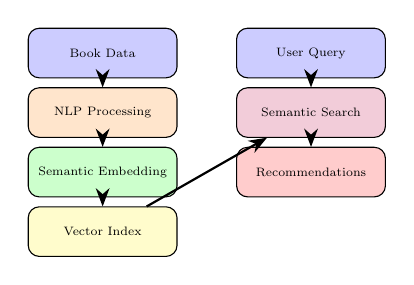
\begin{tikzpicture}[node distance=1.2cm, scale=0.9, every node/.style={font=\scriptsize}, scale=0.7, transform shape]
    % Simplified final architecture
    \node (data) [block, fill=blue!20] {Book Data};
    \node (process) [block, below of=data, fill=orange!20] {NLP Processing};
    \node (embed) [block, below of=process, fill=green!20] {Semantic Embedding};
    \node (index) [block, below of=embed, fill=yellow!20] {Vector Index};
    
    \node (query) [block, right of=data, xshift=3cm, fill=blue!20] {User Query};
    \node (search) [block, below of=query, fill=purple!20] {Semantic Search};
    \node (results) [block, below of=search, fill=red!20] {Recommendations};

    \draw [arrow] (data) -- (process);
    \draw [arrow] (process) -- (embed);
    \draw [arrow] (embed) -- (index);
    \draw [arrow] (query) -- (search);
    \draw [arrow] (index) -- (search);
    \draw [arrow] (search) -- (results);
    \end{tikzpicture}

    \vspace{0.4cm}
    \textbf{Impact \& Applications:}
    \begin{itemize}
      \item Educational tool for privacy-aware ML
      \item Foundation for local-first recommendation systems
      \item Demonstrates transformer accessibility on consumer hardware
    \end{itemize}
  \end{column}
\end{columns}

\end{frame}
\begin{frame}{End of Presentation}
  \centering
    \Large Thank you for your attention!
    \vspace{0.1cm}
    \begin{center}
        \includegraphics[scale=0.4]{figures/tm-logo-nobg-quarter.png}
    \end{center}
    \Large Questions?
\end{frame}

% Backup slides for Q&A
\begin{frame}{Backup: Per-Category Metrics}

\begin{center}
  \includegraphics[width=0.45\textwidth]{refine_category_metrics_plot.png}
\end{center}

\end{frame}

\begin{frame}{Backup: Fallback Keywords}

\begin{itemize}
    \item Fallback used when zero-shot model confidence was low
    \item Example keywords:
    \begin{itemize}
        \item \textbf{Fantasy}: magic, wizard, dragon
        \item \textbf{Science Fiction}: space, AI, dystopia
        \item \textbf{Love}: romance, passion, relationship
        \item \textbf{Mystery}: detective, clue, crime
        % Add more if you like
    \end{itemize}
\end{itemize}

\end{frame}

\begin{frame}{Backup: Performance}

\begin{itemize}
    \item Embedding time per book: $\approx$ 2 ms (batch embedding)
    \item Query embedding: $\approx$ 50-200 ms
    \item FAISS search: $<$ 10 ms
    \item UI render time: $\approx$ 1-2 seconds (including image loading)
    \item All processing fully local on consumer-grade laptop
\end{itemize}

\end{frame}

\begin{frame}{Backup: Concrete Examples}

\begin{columns}[T]
  \begin{column}{0.50\textwidth}
    \textbf{Example Query 1:}
    \begin{beamercolorbox}[sep=4pt,left]{block body}
     \textit{"Books about artificial intelligence and ethics"}
    \end{beamercolorbox}
    
    \textbf{Top Results:}
    \begin{itemize}
      \item  "The Alignment Problem" - Brian Christian
      \item  "Life 3.0" - Max Tegmark  
      \item  "Weapons of Math Destruction" - Cathy O'Neil
    \end{itemize}

    \vspace{0.1cm}
    \textbf{Example Query 2:}
    \begin{beamercolorbox}[sep=4pt,left]{block body}
     \textit{"mystery novels with unreliable narrators"}
    \end{beamercolorbox}
    
    \textbf{Top Results:}
    \begin{itemize}
      \item  "Gone Girl" - Gillian Flynn
      \item  "The Girl on the Train" - Paula Hawkins
      \item  "In the Woods" - Tana French
    \end{itemize}
  \end{column}

  \begin{column}{0.45\textwidth}
    \textbf{What This Demonstrates:}
    \begin{itemize}
      \item  \highlight{Semantic understanding} beyond keywords
      \item  \highlight{Abstract concept matching} (ethics, unreliable narrators)
      \item  \highlight{Cross-genre discovery} potential
    \end{itemize}

    \vspace{0.1cm}
    \textbf{Evaluation Challenges:}
    \begin{itemize}
      \item  No ground truth for "perfect" recommendations
      \item  Subjective nature of book preferences
      \item  \highlight{Solution:} Focus on semantic relevance rather than prediction accuracy
    \end{itemize}

    \vspace{0.1cm}
    \textbf{Discussion Starters:}
    \begin{itemize}
      \item  How could one evaluate recommendation quality
      \item  Books with sparse descriptions
      \item  Could this approach work for other domains?
    \end{itemize}
  \end{column}
\end{columns}

\end{frame}

\end{document}